\Chapter{An Artist Abroad}{Glyn Court}

My mother had always promised herself that when she had a garden of her own there would be a little stream purling through and adding its liquid music to the scents and colours of the flowers; but my father thought differently: he had too keen a recollection of the floods which time and again had swept down the valley and inundated his boyhood home; so when, on his marriage, he moved from Roadwater to Washford he chose the site for his new house on the hillside.

His land was a quarter of an acre of orchard, with various buildings, and half an acre of vegetable gardens attached to three ancient cottages. This garden sloped down on the west to a cutting of the abandoned West Somerset Mineral Railway, while along the northern boundary ran the main road from Minehead to Taunton, which had been raised sixty years before to cross the railway by a ramp and now ran level with the eaves of the cottages. Mother soon had a garden and cultivated it happily, but it was not everything she desired, for so much of the land was cultivated by others, and her flowers and shrubs needed room to grow and blossom freely. She had to wait - fifteen years, I guess, for even if room had opened up, times were difficult, hours were long, leisure was short, and living was hard.

Father was distressed that she could not have the garden of her heart, and that he could not provide one of the few things that she, undemanding soul, would have loved to have; but within the limitations of space and time he would do all that imagination and hard work could achieve. 

Gardeners, like poets, are born, not made, and the poetry of his sensitive nature went into his strong, stubby craftsman's hands. When the desire to create came upon him - and it frequently did - he expressed it not in words but in the works of those hands; and they took an astonishing variety of forms. Moreover, his own taste in gardening, like my mother's, ran toward the beautiful and decorative rather than the utilitarian: he would rather build ten flower gardens than dig one vegetable plot.

I hardly need say that this was not indolence on his part. Hard work and he had never fallen out. They were lifelong acquaintances and the best of friends; but after a few early struggles with a spade and a bizgy in his father's garden he had decided that, inscrutable though most of the decrees of Providence might be, one of them was clear as crystal: that he was not meant to be a gardener and he held firmly to this article of faith.

During the war years, when the broadcasts of those hortatory horticulturalists the Radio Doctor and Mr Middleton made us acutely conscious of the need to grow more food, the vegetable garden was painstakingly mapped out and seeded and raked and hoed and scuffled, but it was generally the current Bob or Graham or other lad of pre-military age who performed the surgery.

I will not say that my father never gardened, but his distaste for it was made strikingly evident when that health-giving exercise known in the classic tongue as \quotemark{spittin' up a rap for the teddies} was entrusted to the proven and many-sided incompetence of his sixteen-year old son. But to make a garden, to create an outdoor home, to see those lawns, paths, flower-beds and ponds conceived in the imagination, gradually being clothed in the garments of colour and shapeliness and liquid light, there was work for the artist that he was and would never have claimed to be. And another incentive, perhaps even stronger for him, was the delight in the garden my mother found as soon as she had one of her own and as soon as the opportunity came he set to work with all his vigour to build her an ornamental garden to complete the home he thought she deserved. But eventually, and suddenly, the opportunity came. The old couple in one of the cottages died and their daughter moved away; and another cottage was made uninhabitable by fire. So my father, much as he loved old for old's sake, demolished them, and the stones and cob of which they were made went, some of them, back into the earth, but far more - and here Father seized his opportunity - went to make mother's garden.

I have spoken of the old country virtue of thrift, economy, making do, never throwing away, using thrice over, but it comes as a surprise - and raises a chuckle - to find the creative gardener just as ardent an economist as the carpenter or the shoemaker. After all, his raw material is reasonably cheap.

The cottages had stood in a hollow, pitched with cobbles, between the embanked vegetable garden and the raised level of the road, but the rough debris raised the ground by three feet and on the site of the cottages he laid out a triangle of lawn with a sunken rose garden. But after all that, an incredible quantity of building materials remained over, and every item bore the marks of its history: roof trees hewn with the adze and notched and numbered to take the roughly sawn rafters; wall-plates and joists studded with nails and brads forged by a sixteenth-century blacksmith; heavy doors with massive locks nearly a foot square; oak floorboards from the bedrooms, hand sawn three centuries before, not squared off but left in the shape of the trunk of the tree; red chimney bricks of more modern date; quarry tiles which had, as a luxury, replaced the beaten earth floor downstairs; incongruously, a few bright glossy red tiles from the Victorian fireplace; and stones ... ah! The stones, of every weight from a pound to a hundredweight, red sandstone, yellow sandstone, blue lias boulders, Doulting stone ... there seemed no end to their variety. A curious philosopher might have wondered why a Jacobean builder, forced to fetch and carry by pack-horse over ways that were quagmires, should have gone to seven or eight widely separated quarries for stones for three small cottages but on looking more closely he would have seen what soon became apparent to us as well: that one huge quarry provided these stones, the Cistercian monastery two fields away, for we could see that many of them had been shaped by the mason's chisel; there were sandstone segments which had gone to form the massive pillars of the church; quoins and chamferings of Doulting stone; stone from mullions; and it all taught a piquant lesson in social history: that whereas many of the leading families of the realm owed their prosperity to an unscrupulous pillager of the Church, honest Hodge was not slow to follow where Marprelate led.

The stones served a multitude of uses: paving, edging to new flower beds, building retaining walls, rockeries, ornamental steps: some of the best square-cut stones went to make a fine upping-block, though by that time father was unlikely to acquire anything much more equine than a new Hudson or a hobby horse.

From the oaken king-posts and cross beams he made a gateway, capped with the coping tiles, and, in the garden, a little shingle-roofed summerhouse in which they would sit on Sunday evenings in summer looking down over the fields to the stream and the hills beyond.

But the most distinctive creations were from the most unpromising material, the red brick of the cottage chimneys. He thought that, even if Ada could not have a stream in the garden, he would give her the next best thing, and just over the hedge of the house lawn, in the cottage garden where the rows of kidney beans had stood, he constructed an ornamental pond, roughly in the shape of a harp, with arms curving round the foot of an old apple tree - a Tom Putt, I think. He took great pains to seal the floor, and - again economically! - set the concrete of the sides to harden behind shields of flattened oil drums ... And to this day, if you look hard, you may see imprinted the cabalistic sign.

\begin{figure}[]
	\centering
     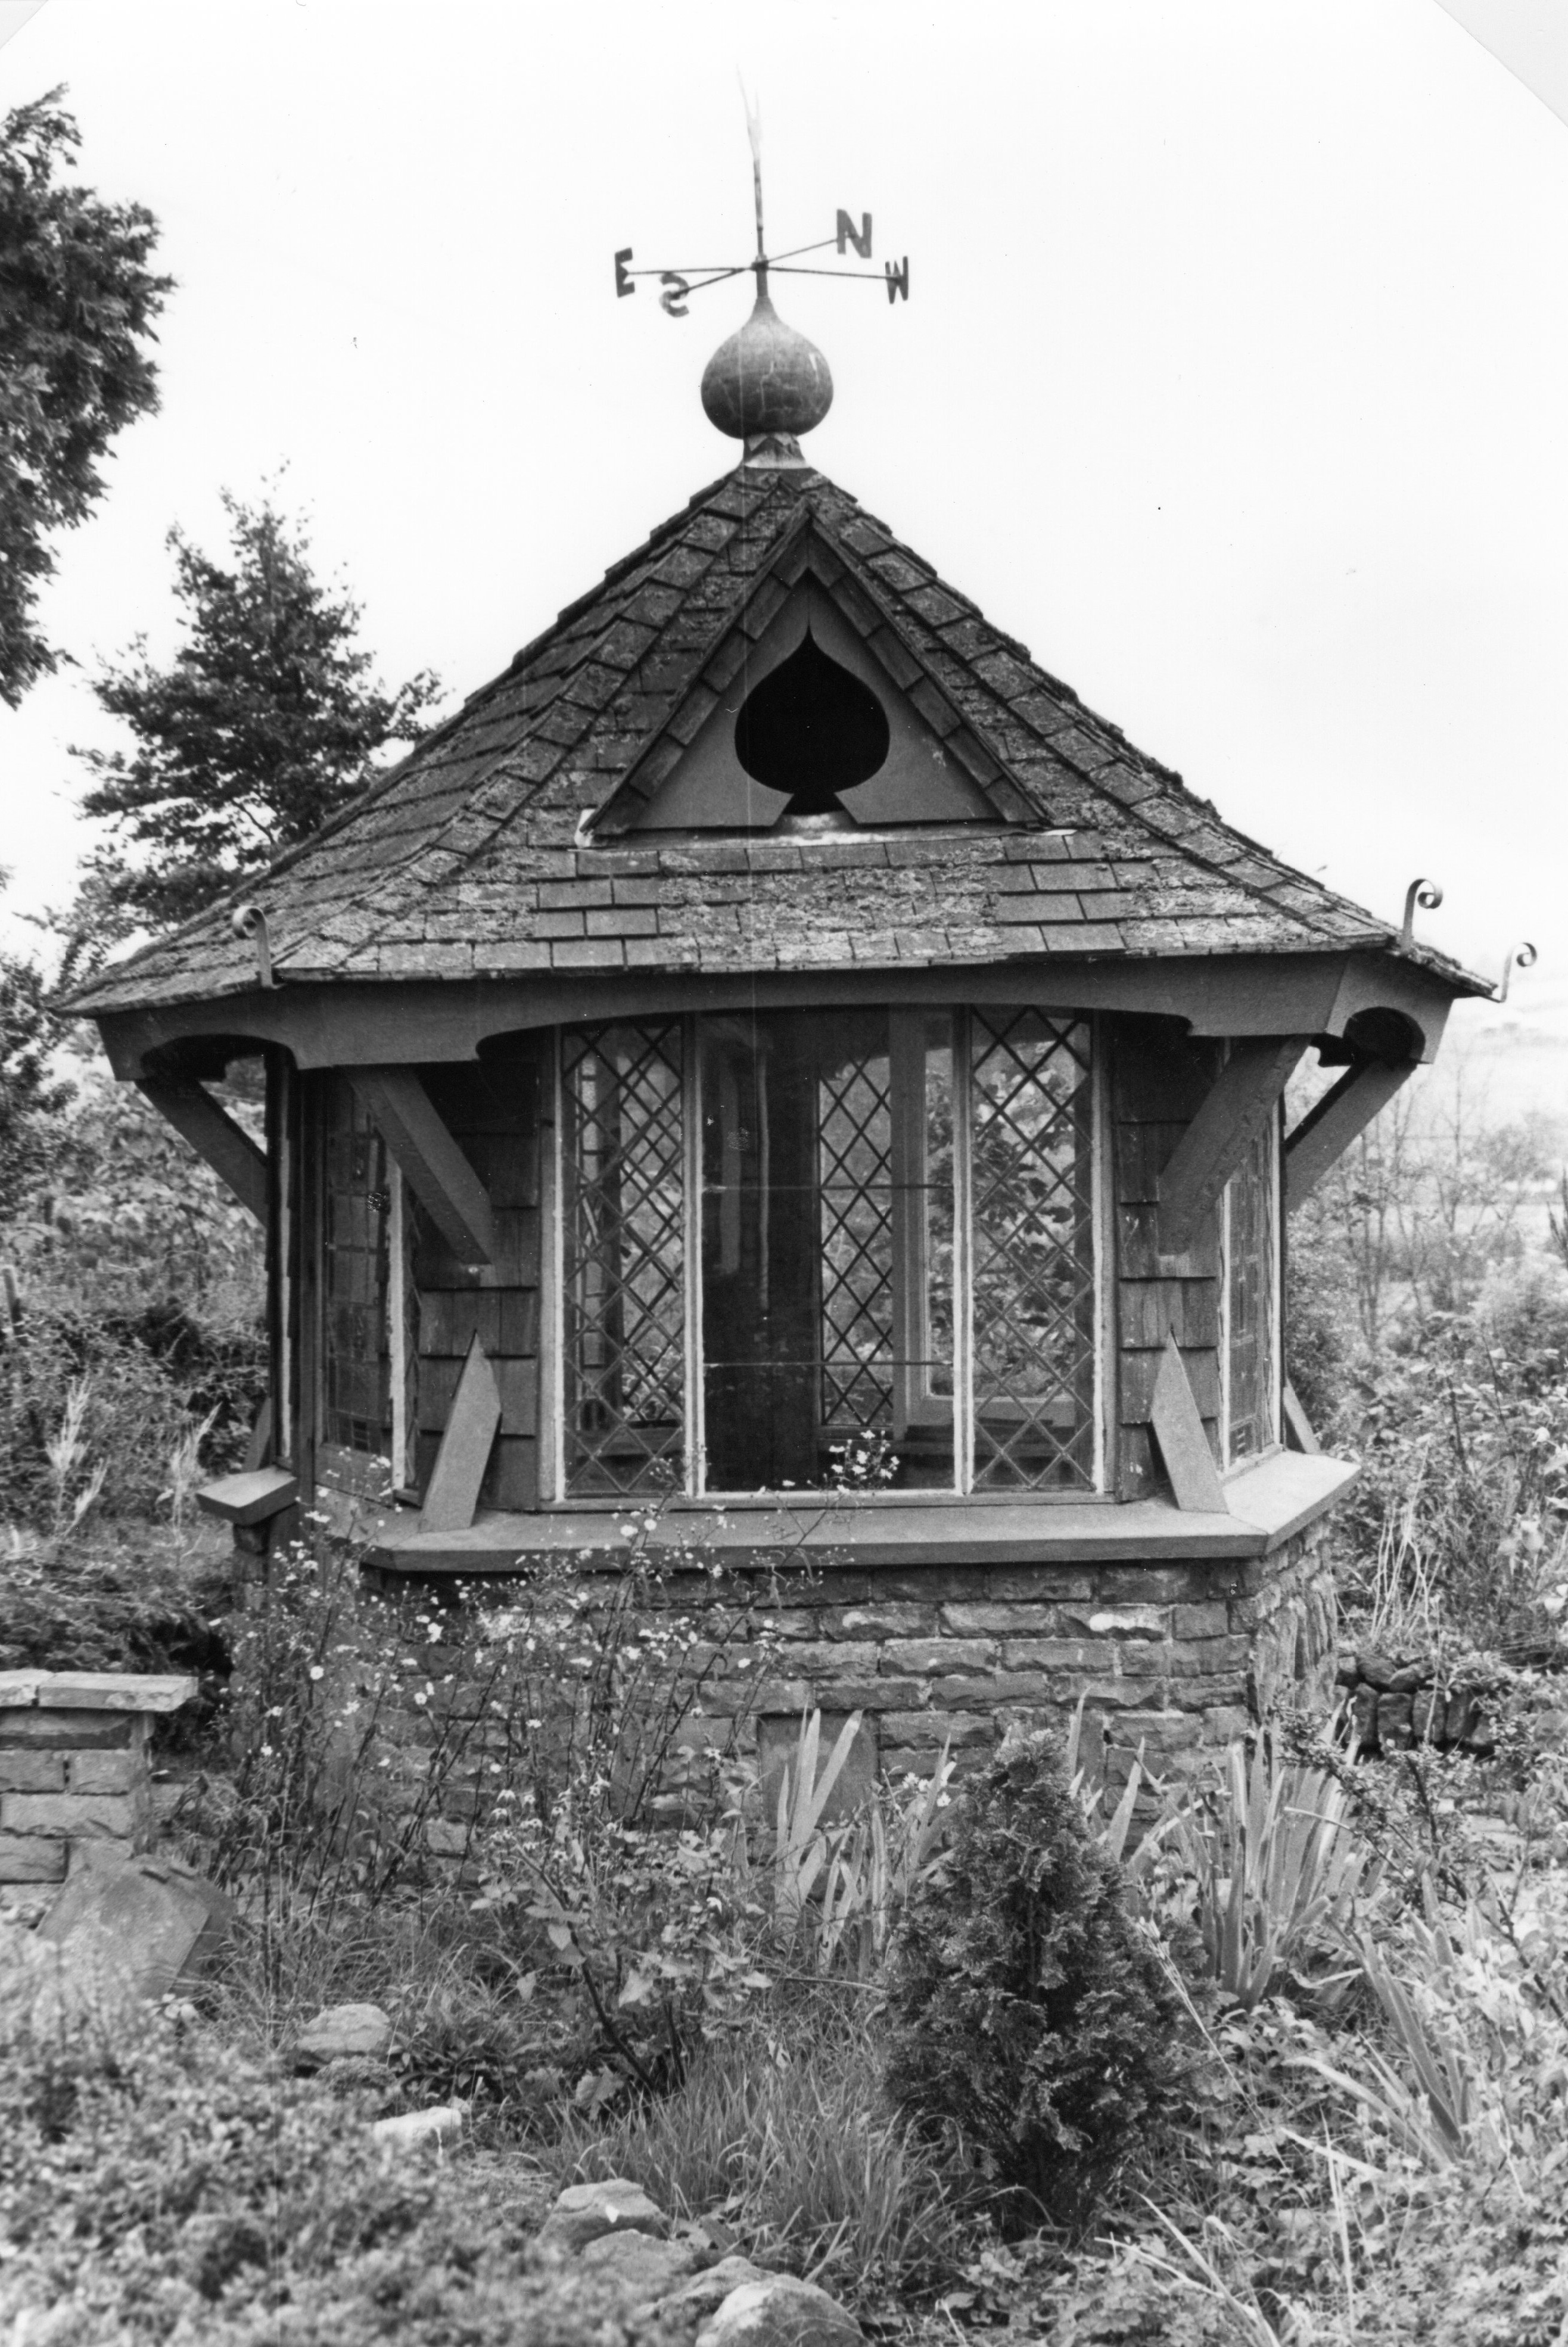
\includegraphics[width=1\textwidth]{figures/Summerhouse}
     \caption{The Summerhouse. Built in a similar pentagonal design to that of Dunster Market}
     \label{fig:SummerHouse}
\end{figure}


Over the lower end of the pond he constructed a little bridge of bricks set alternately flat and on end in a cap and gap pattern, with a mosaic foot-way, and although worn away here and there it is as strong as on the day he made it. Typically, though, he would not use a sharp-edged brick anywhere, but very carefully and laboriously chipped off every edge of every brick before he set it in place.

But his triumph of improvisation was the summerhouse. Father had always loved the picturesqueness of our unspoilt villages, of which the epitome, in many ways, was Dunster; and the jewel of Dunster village is the seventeenth century yarn market. Father took it as his model, but it was not in him to copy anything slavishly, and the construction was uniquely his own.

The ground-plan of the yarn market is a hexagon, a geometrical figure which is both easy to construct and pleasant to contemplate; the one which best combines the qualities of the strength of the rectangle with the grace of the circle. This regularity would not do for Father. It was easy to achieve, and therefore probably meretricious and suspect. So in a cement base he laid down the foundations of a five sided summerhouse.

This is a simple enough calculation for a geometrician, but Father knew nothing of interior angles, and sums of right angles and suchlike arcana and his projector and theodolite were a spirit level and a two foot rule or a length of string, and several pounds' weight of patience; so that the plotting of the summerhouse seems to me worth recording.

Having said that, I must go further and confess that it is only since beginning this chapter that I have looked at the summerhouse closely, and only now that I have realised the reason for its proportions. Everything was built round the windows! Some time before this, from a journey to Wedmore - unforgettable to them because the apple orchards were seas of blossom - he and mother had brought back a miscellaneous collection of stained glass windows, diamond panes and leaded lights, and at last he had found a proper use for them. So the lights flanked by diamond panes, determined the length of the sides.

At his five corners he dug holes three feet deep and planted sleepers from the local branch line of the G.W.R. Four of the sides he then filled in nearly up to waist-level with his hewn-edged bricks, but even here he aimed for unobtrusive variety: two of the sides, the three lowest courses and below the three topmost, are set in a pattern of blocks of three, alternately vertical and horizontal, with a clay tile from the cottage floor inserted centrally rather as a bas relief: those seen from the garden are set in his beloved herringbone pattern, and the square tile has become a diamond.

On each of the top courses he placed a sill, curved on the inside to form a simple decorative ledge, and on these he set the lights, which filled in the whole space to the top of the posts. The fifth side took the door of his favourite double or stable door type, the lower half made of light oaken boards of irregular shapes cunningly tongued and grooved, the upper half a partly coloured leaded light set in an oaken frame.

With joists and boards from the cottages he made the pentagonal roof, and he clad it with shingles, out over one window he constructed a gable with a light shaped like a formalized ivy leaf. On the summit he placed a cone of cement, like a visual echo of the ivy leaf, and he crowned the whole structure with a weathercock, a confident, challenging bird. He was most carefully drawn for balance and cut out by hand from a sheet of copper and he has stood up to the storms of more than thirty winters. In my heady youth, an occasional apple core was hurled to see how fast the fickle fowl would revolve, but he has borne up bravely, gyrating on bicycle ball-bearings, and he is still pert and lively enough to have served as a model for Milton's roystering rooster who \\
…with lively din \\
Scatters the rear of darkness thin.\\

All round and within the summerhouse Father laid in a pattern the red tiles which perfectly complement the brick, and as a finishing touch he fixed swivel seats - post office sorters' seats - to the uprights, and the little pleasure-dome was ready for every modest festivity to which the soft summer days would invite.

Of course, much as he loved plain wood, he bowed to the necessity of paint for outdoor work; but at least five years before, he had bought a two-gallon tin of orange chrome paint and only used a pint on the garage door; so it was brought out of retirement, put into service for the window sills - and it is as cheerful a colour as heart could desire - and then it was laid back into store in the Aladdin's cave of a workshop. There it matured and increased in virtue and strength, until, thirty-five years later, I gave the window sills a second coat, and by that time the orange chrome would not have disgraced the palette of Veronese himself.